\section{研究背景}
\subsection{背景说明}
在校园面积较大的高校,师生通常会使用代步工具包括自行车、电瓶车、电动滑板等进行校园内通勤。电瓶车、电动滑板需要定期进行充电,而将电瓶带入宿舍或是从宿舍拉电线的充电行为有极大的安全隐患,被高校明令禁止。为解决师生充电困难问题,校方通常会在校园开阔地带建设固定充电桩。\\
\indent 以成电清水河校区为例,经调查校园现有15个充电点位,每个充电点位可同时容纳24辆电动自行车充电。分布情况如图所示:
\begin{figure}[H]
    \centering
    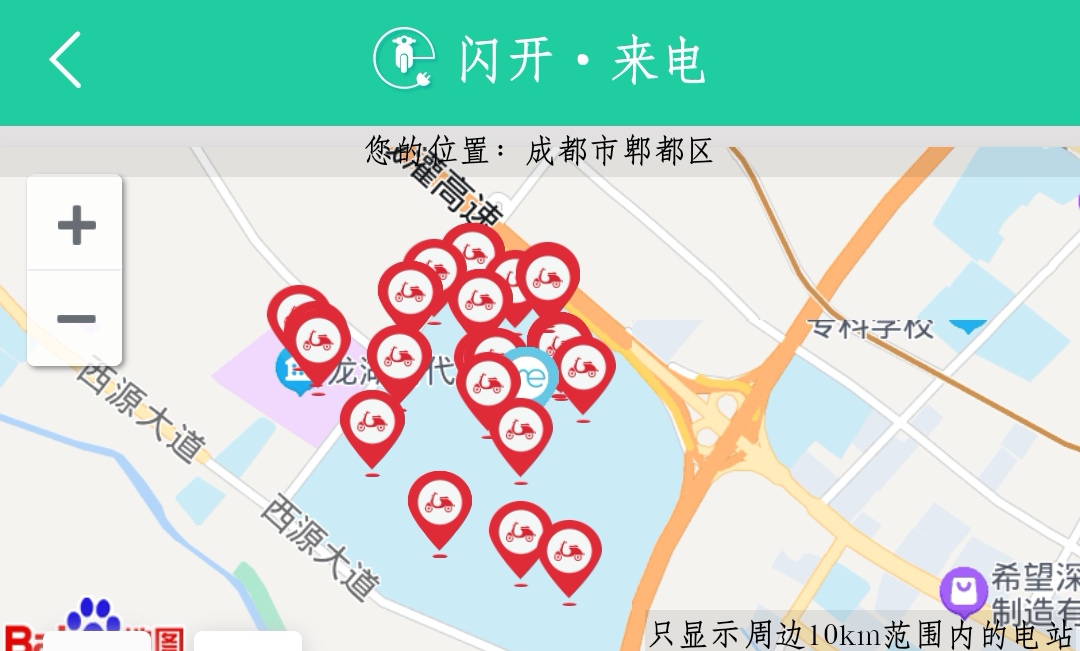
\includegraphics[width=0.6\textwidth]{pic1.jpg}
    %\caption{自卸车卸货的两个过程}
    \caption{闪开来电校园充电桩分布}
\end{figure}
但是在校园论坛中我们发现同学们对于设置地点与充电口数目不合理的抱怨。比如,充电桩离自己常去的地方过远,来往于充电路途非常花时间;充电桩数目过少,不易寻找到空闲位置……\\
\indent 对于上述问题,我们认为对于充电桩建设点位进行规划可以减缓同学的抱怨。什么地方可以建设充电桩,在什么地方建设充电桩会更好。\\
\indent 我们对校园内环境进行了调研,我们归纳出包括但不限于现有充电桩的30个可建设充电桩位置.(\textit{基本要求:空余面积不小于15$m^2$、附近可接入电源、满足一定人流量})
\subsection{研究目标}
那么在固定充电桩设置地点与充电口数目的情况下,校方对于充电桩的选址是否最优,如果不是最优选址,那么最优选址应该被定在哪里。以及在每一个充电桩应该预留多少个充电口引起了我们的好奇,我们希望能通过运筹学的方式得到问题的解答。






